\Section{Algebra practice---graph interpretation}

The figure below shows the graph of the function $f$.

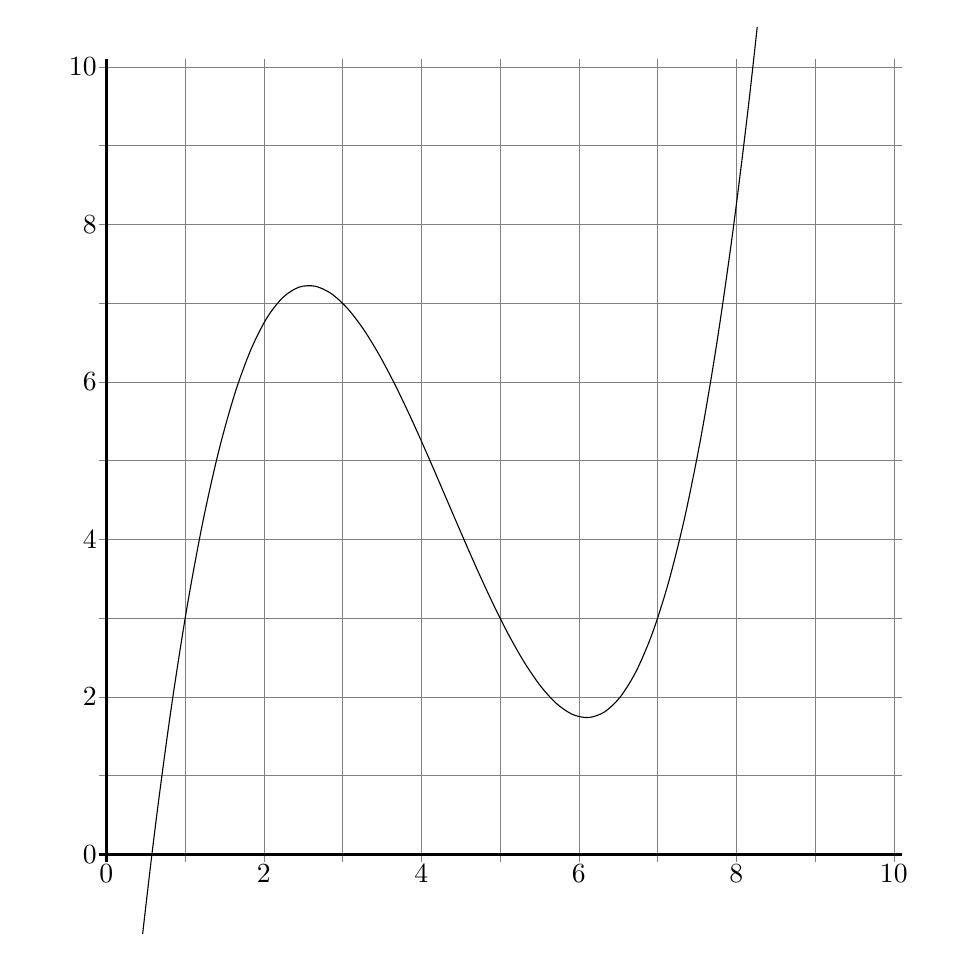
\begin{tikzpicture}
 \clip
 (-1,-1) rectangle (10.5,10.5)
 ;
 \draw[very thin,color=gray] (-0.1,-0.1) grid (10.1,10.1);
 \draw
 (0,0) node[below] {0}
 (2,0) node[below] {2}
 (4,0) node[below] {4}
 (6,0) node[below] {6}
 (8,0) node[below] {8}
 (10,0) node[below] {10}
 (0,0) node[left] {0}
 (0,2) node[left] {2}
 (0,4) node[left] {4}
 (0,6) node[left] {6}
 (0,8) node[left] {8}
 (0,10) node[left] {10}
 ;
 \draw[thick] (-0.1,0) -- (10.1,0);
 \draw[thick] (0,-0.1) -- (0,10.1);
 \draw
 plot[very thick, domain=0:10, range=0:10, smooth, samples=50]
 (\x, {0.25*(\x - 1)*(\x - 5)*(\x - 7) + 3})
 ;
\end{tikzpicture}

\begin{ProblemSet}[pencil space=0.75in]
 \begin{Problem}
  What is $f(3)$?
 \end{Problem}
 \begin{Problem}
  What are the solutions to $f(x) = 3$?
 \end{Problem}
 \begin{Problem}
  What is $f(4)$?
  Give an approximation to about the nearest tenth.
 \end{Problem}
 \begin{Problem}
  What are the solutions to $f(x) = 6$?
  Give an approximation to about the nearest tenth.
 \end{Problem}
\end{ProblemSet}

%%% Local Variables:
%%% mode: latex
%%% TeX-master: "Business-calculus-workbook"
%%% End:
